
\documentclass[tikz]{standalone}

\begin{document}
\tikzset{man/.pic={
    \node[circle,fill,minimum size=5mm] (head) {};
    \node[rounded corners=2pt,minimum height=.8cm,minimum width=0.4cm,fill,below = 1pt of head] (body) {};
    \draw[line width=1mm,round cap-round cap] ([shift={(2pt,-1pt)}]body.north east) --++(-90:6mm);
    \draw[line width=1mm,round cap-round cap] ([shift={(-2pt,-1pt)}]body.north west)--++(-90:6mm);
    }}
\begin{tikzpicture}
    % \node[align=center] (0) at (0, 3) {\textbf{Prisoner's Dilemma}};

    \pic[solarizedGreen] at (.5, -.5) (myman) {man};
    \node[align=center] (0) at (3, 0) {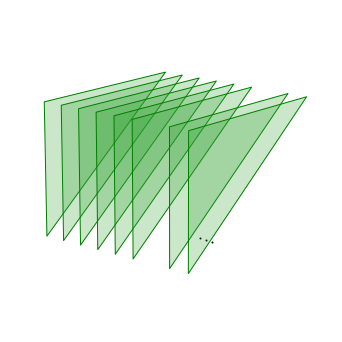
\includegraphics[width=.3\textwidth]{static/reactive_n.png}};

    \coordinate  (A) at (.5, 0);
    \coordinate  (B) at (1.5, .5) ;
    \draw [->, thick] (A.north) to [out=90,in=180] (B.north);
\end{tikzpicture}
\end{document}